\section{Software: Hawen}
\label{sec:WP4:Hawen:software}

\begin{table}[h!]
    \centering
    { \setlength{\parindent}{0pt}
    \def\arraystretch{1.25}
    \arrayrulecolor{numpexgray}
    {\fontsize{9}{11}\selectfont
    \begin{tabular}{!{\color{numpexgray}\vrule}p{.4\textwidth}!{\color{numpexgray}\vrule}p{.6\textwidth}!{\color{numpexgray}\vrule}}
        \rowcolor{numpexgray}{\rule{0pt}{2.5ex}\color{white}\bf Field} & {\rule{0pt}{2.5ex}\color{white}\bf Details} \\
        \rowcolor{white}\textbf{Consortium} & \begin{tabular}{l}
Inria\\
\end{tabular} \\
        \rowcolor{numpexlightergray}\textbf{Exa-MA Partners} & \begin{tabular}{l}
Inria BXSO\\
\end{tabular} \\
        \rowcolor{white}\textbf{Contact Emails} & \begin{tabular}{l}
florian.faucher@inria.fr\\
\end{tabular} \\
        \rowcolor{numpexlightergray}\textbf{Supported Architectures} & \begin{tabular}{l}
CPU Only\\
\end{tabular} \\
        \rowcolor{white}\textbf{Repository} & \href{https://gitlab.com/ffaucher/hawen}{https://gitlab.com/ffaucher/hawen} \\
        \rowcolor{numpexlightergray}\textbf{License} & \begin{tabular}{l}
OSS:: GPL v*\\
\end{tabular} \\
        \rowcolor{white}\textbf{Bottlenecks roadmap} & \begin{tabular}{l}
B10 - Scientific Productivity\\
B11 - Reproducibility and Replicability of Computation\\
B6 - Data Management\\
B7 - Exascale Algorithms\\
\end{tabular} \\
        \bottomrule
    \end{tabular}
    }}
    \caption{WP4: Hawen Information}
\end{table}

\subsection{Software Overview}
\label{sec:WP4:Hawen:summary}

\hawen~solves quantitative inverse wave problem by following 
and iterative minimization approach, \cite{Faucher2020adjoint,faucher_hawen_2021}.
The sketch of the iterative procedure is depicted 
in \cref{figure:hawen:wp4:inversion}, and is typically a 
Newton-type nonlinear optimization approach, \cite{Virieux2009}.
This procedure heavily relies onto numerical simulations of 
wave propagation, which are compared with the data at each 
iteration. Therefore, an efficient modeling solver is required,
it is investigated in WP1 for \hawen, \cref{sec:WP1:Hawen:software}.
In addition, investigation regarding the choices of the acquisition
(to limit the number of sources to use) and the on efficient criterion
to evaluate the discrepancy between the data and the simulations 
are necessary to reduce the computational cost.

In~\cref{tab:WP4:Hawen:features} we provide a summary of the software features relevant to the work package which are briefly discussed.

\begin{figure}[ht!]\centering
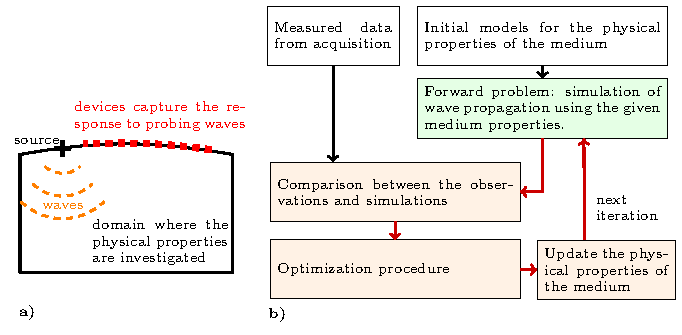
\includegraphics[scale=1.00]{graphics/hawen/haven_inversion}
\caption{Sketch of the quantitative inverse wave problems based upon 
         iterative minimization in \hawen. %, extracted from \cite{faucher_hawen_2021}. 
         \textbf{a)} Acquisition stage: probing waves are are 
                     recorded by devices positioned on a portion 
                     of the domain, typically near the boundary.
         \textbf{b)} The reconstruction algorithm starts from initial 
                     model parameters and compares simulations of wave
                     propagation with the data, 
                     then iteratively updates those properties using
                     a Newton-based algorithm.}
\label{figure:hawen:wp4:inversion}
\end{figure}


\begin{table}[h!]
    \centering
    { 
        \setlength{\parindent}{0pt}
        \def\arraystretch{1.25}
        \arrayrulecolor{numpexgray}
        {
            \fontsize{9}{11}\selectfont
            \begin{tabular}{!{\color{numpexgray}\vrule}p{.25\linewidth}!{\color{numpexgray}\vrule}p{.6885\linewidth}!{\color{numpexgray}\vrule}}
    
    \rowcolor{numpexgray}{\rule{0pt}{2.5ex}\color{white}\bf Features} &  {\rule{0pt}{2.5ex}\color{white}\bf Short Description }\\ 
    
\rowcolor{white}    deterministic inverse problem & provide short description here \\
\end{tabular}
        }
    }
    \caption{WP4: Hawen Features}
    \label{tab:WP4:Hawen:features}
\end{table}


\subsection{Parallel Capabilities}
\label{sec:WP4:Hawen:performances}


\hawen~uses MPI and OpenMP parallelism. The HDG method is particularly 
appropriate for parallelism (as other methods in the DG family), such 
that each cell of the mesh can be treated independently in parallel. 
\hawen~has been used on several supercomputers, including GENCI Adastra
with Genoa partition for CPUs parallelism.
\hawen~is linked with MUMPS library, which is a multifrontal direct solver 
for sparse linear systems. 
MUMPS allows to solve for multiple right-hand side, hence reducing the 
computational cost of having many sources in the acquisition during 
inversion.

%\begin{itemize}
%    \item describe the parallel programming  environment : MPI, OpenMP, CUDA, OpenACC, etc.
%    \item describe the parallel computation environment: type of architecture and super computer used.
%    \item describe the parallel capabilities of the software
%    \item \textbf{Scalability:} Describe the general scalability properties of the software
%    \item \textbf{Integration with Other Systems:} Describe how the software integrates with other numerical libraries in the Exa-MA framework.
%\end{itemize}


\subsection{Initial Performance Metrics}
\label{sec:WP4:Hawen:metrics}


The performance of inversion can be evaluated with different
criteria. 
It typically is a compromise between the accuracy (resolution) 
of the final reconstruction and the computational cost required
to reach it. 
The number of iterations and complexity of the computations involved 
at each of them is also a criterion for numerical efficiency.
We also wish to investigate target-oriented inversion, to reconstruct
some part of the model without having to simulate everything, hence
reducing the computational cost.


%This section provides a summary of initial performance benchmarks performed in the context of WP4. It ensures reproducibility by detailing input/output datasets, benchmarking tools, and the results. All data should be publicly available, ideally with a DOI for future reference.
%
%\begin{itemize}
%    \item \textbf{Overall Performance:} Summarize the software's computational performance, energy efficiency, and scalability results across different architectures (e.g., CPU, GPU, hybrid systems).
%    \item \textbf{Input/Output Dataset:} Provide a detailed description of the dataset used for the benchmark, including:
%        \begin{itemize}
%            \item Input dataset size, structure, and format (e.g., CSV, HDF5, NetCDF).
%            \item Output dataset format and key results.
%            \item Location of the dataset (e.g., GitHub repository, institutional repository, or open access platform).
%            \item DOI or permanent link for accessing the dataset.
%        \end{itemize}
%    \item \textbf{open-data Access:} Indicate whether the datasets used for the benchmark are open access, and provide a DOI or a direct link for download. Where applicable, highlight any licensing constraints.
%    \item \textbf{Challenges:} Identify any significant bottlenecks or challenges observed during the benchmarking process, including data handling and computational performance.
%    \item \textbf{Future Improvements:} Outline areas for optimization, including dataset handling, memory usage, or algorithmic efficiency, to address identified challenges.
%\end{itemize}

\subsubsection{Benchmark \#1: Visco-acoustic time-harmonic wave propagation}
\label{subsec:WP4:Hawen:benchmark1}


\paragraph{Description}
The configuration for the inversion investigated in this benchmark
is based upon the related benchmarks of \hawen~of WP1 and WP3, 
respectively \cref{subsec:WP1:Hawen:benchmark1,subsec:WP3:Hawen:benchmark1}.
Here we use the acoustic case, and our target model is the one 
given in \cref{figure:hawen:seam-model}.
For the reconstruction, we will take a smooth representation of the 
model, and vary the degree of smoothness to make the reconstruction 
harder. 

\paragraph{Input/Output Dataset Description}
The input data for inversion consist in the recording 
of waves near the boundary for different position of 
sources, as illustrated in the panel a) 
of \cref{figure:hawen:wp4:inversion}. We will use 
synthetically generated wave, and add noise to our data-set. 
In addition, we can provide different acquisition setup, 
i.e., varying the number of sources and number of data-points.


\paragraph{Results Summary}
The accuracy of the reconstruction will be evaluated depending
on the number of iterations required. We will also try to use 
target-oriented inversion to limit the computational cost by 
only inverting part of the domain. 
In this case some well-designed discrepancy criterion can be 
employed to fully use the data-set, cf. our previous works in
\cite{Faucher2019FRgWIGeo,Faucher2020DAS}.

%\begin{itemize}
%    \item \textbf{Description:} Briefly describe the benchmark case, including the problem size, target architecture (e.g., CPU, GPU), and the input data. Mention the specific goals of the benchmark (e.g., testing scalability, energy efficiency).
%    \item \textbf{Benchmarking Tools Used:} List the tools used for performance analysis, such as Extrae, Score-P, TAU, Vampir, or Nsight, and specify what metrics were measured (e.g., execution time, FLOPS, energy consumption).
%    \item \textbf{Input/Output Dataset Description:}
%        \begin{itemize}
%            \item \textbf{Input Data:} Describe the input dataset (size, format, data type) and provide a DOI or link to access it.
%            \item \textbf{Output Data:} Specify the structure of the results (e.g., memory usage, runtime logs) and how they can be accessed or replicated.
%            \item \textbf{Data Repository:} Indicate where the data is stored (e.g., Zenodo, institutional repository) and provide a DOI or URL for accessing the data.
%        \end{itemize}
%    \item \textbf{Results Summary:} Include a summary of key metrics (execution time, memory usage, FLOPS) and their comparison across architectures (e.g., CPU, GPU).
%    \item \textbf{Challenges Identified:} Describe any bottlenecks encountered (e.g., memory usage, parallelization inefficiencies) and how they impacted the benchmark.
%\end{itemize}


\subsubsection{Benchmark \#2: Visco-elastic time-harmonic wave propagation}
\label{subsec:WP4:Hawen:benchmark2}

This benchmark will be similar to the above but considering elastic medium,
hence drastically increasing the computational cost. For inversion and 
additional difficulty lies in that more model parameters need to be reconstructed,
hence increasing the uncertainties and difficulties.

\subsection{12-Month Roadmap}
\label{sec:WP4:Hawen:roadmap}

We wish to combine the results of WP1 and WP3 
\cref{sec:WP1:Hawen:software,sec:WP3:Hawen:software} 
to obtain the most efficient configuration for inversion.
Once the numerical setup is designed, everything will be 
made available on a dedicated repository for reproducibility.


%In this section, describe the roadmap for improving benchmarks and addressing the challenges identified. This should include:
%\begin{itemize}
%    \item \textbf{Data Improvements:} Plans for improving input/output data management, including making datasets more accessible and ensuring reproducibility through open-data initiatives.
%    \item \textbf{Methodology Application:} Implementation of the benchmarking methodology proposed in this deliverable to streamline reproducibility and dataset management.
%    \item \textbf{Results Retention:} Plans to maintain benchmark results in a publicly accessible repository with appropriate metadata and documentation, ensuring long-term usability.
%\end{itemize}

In~\cref{tab:WP4:Hawen:bottlenecks}, we briefly discuss the bottleneck roadmap associated to the software and relevant to the work package.

\begin{table}[h!]
    \centering
    
    

    \centering
    { 
        \setlength{\parindent}{0pt}
        \def\arraystretch{1.25}
        \arrayrulecolor{numpexgray}
        {
            \fontsize{9}{11}\selectfont
            \begin{tabular}{!{\color{numpexgray}\vrule}p{.25\linewidth}!{\color{numpexgray}\vrule}p{.6885\linewidth}!{\color{numpexgray}\vrule}}
    
    \rowcolor{numpexgray}{\rule{0pt}{2.5ex}\color{white}\bf Bottlenecks} &  {\rule{0pt}{2.5ex}\color{white}\bf Short Description }\\ 
    
\rowcolor{white}    B10 - Scientific Productivity & provide short description here \\
\rowcolor{numpexlightergray}    B11 - Reproducibility and Replicability of Computation & provide short description here \\
\rowcolor{white}    B6 - Data Management & provide short description here \\
\rowcolor{numpexlightergray}    B7 - Exascale Algorithms & provide short description here \\
\end{tabular}
        }
    }
    \caption{WP4: Hawen plan with Respect to Relevant Bottlenecks}
    \label{tab:WP4:Hawen:bottlenecks}
\end{table}
